% Software Development for Mobile Devices
\documentclass[11pt,english,numbers=endperiod,parskip=half]{scrartcl}

\usepackage{color}
\usepackage{graphicx}
\usepackage{minted}
\usepackage{fancyhdr}
\usepackage{pdflscape}
\usepackage{listings}
\usepackage{pifont}
\usepackage{pdfpages}

\newcommand{\cmark}{\ding{51}}

\pagestyle{fancy}

\rhead{Daniel Parker - 971328X}
\lhead{COS30017 - Software Development for Mobile Devices}

\title{Distinction Experience Report}
\subtitle{COS30017 - Software Development for Mobile Devices}
\author{Daniel Parker 971328X}

\date{\today}

\begin{document}
\maketitle
\thispagestyle{empty}

\section{Introduction}
  \centering
    \textbf{Perspective:} Design Communication Perspective

  \raggedright
    This document covers the experience of writing a non-trivial Android
    application from the perspective of communicating the design of the app,
    including class diagrams, navigation model and data model. It also covers
    limitations of API used in developing the program, as well as a short
    section on the experience of using RAPPT for prototyping during initial
    phases of development, and how that affected the continued development.

\section{Project Structure}
  The application is structured in part as per the Android standards, and also
  by how RAPPT has generated package structures and various utilities such as
  RESTful API client, error dialogs, listview and list adapters.

  \subsection{Resources}
    Resources are separated into;
    \begin{itemize}
      \item{anim}
      \item{drawable}
      \item{layou}
      \item{menu}
      \item{values}
    \end{itemize}
    There are different
    styles specified for API 21 than API 15+ due to the need to use the AppCompat
    themes and libraries for backwards compatibility of Material Design components,
    visual and navigation design patterns.

  \subsection{Source}
    Java source is separated as suggested by the output of RAPPT into the following
    packages;
    \begin{itemize}
      \item{activites}
      \item{adapters}
      \item{fragments}
      \item{interfaces}
      \item{model}
      \item{views}
    \end{itemize}
    Some application level source files are in the root of the java source to
    indicate their global importance to the project.

  \subsection{Libraries}
  Most libraries are included by gradle at compile time, however one library
  needed modifications, and has been packaged as a jar archive and added
  to the libs directory and as a gradle dependency.
\section{Program Structure}
\newpage
  \subsection{Class Diagram}
    \begin{figure}[H]
      \centering{
        \fbox{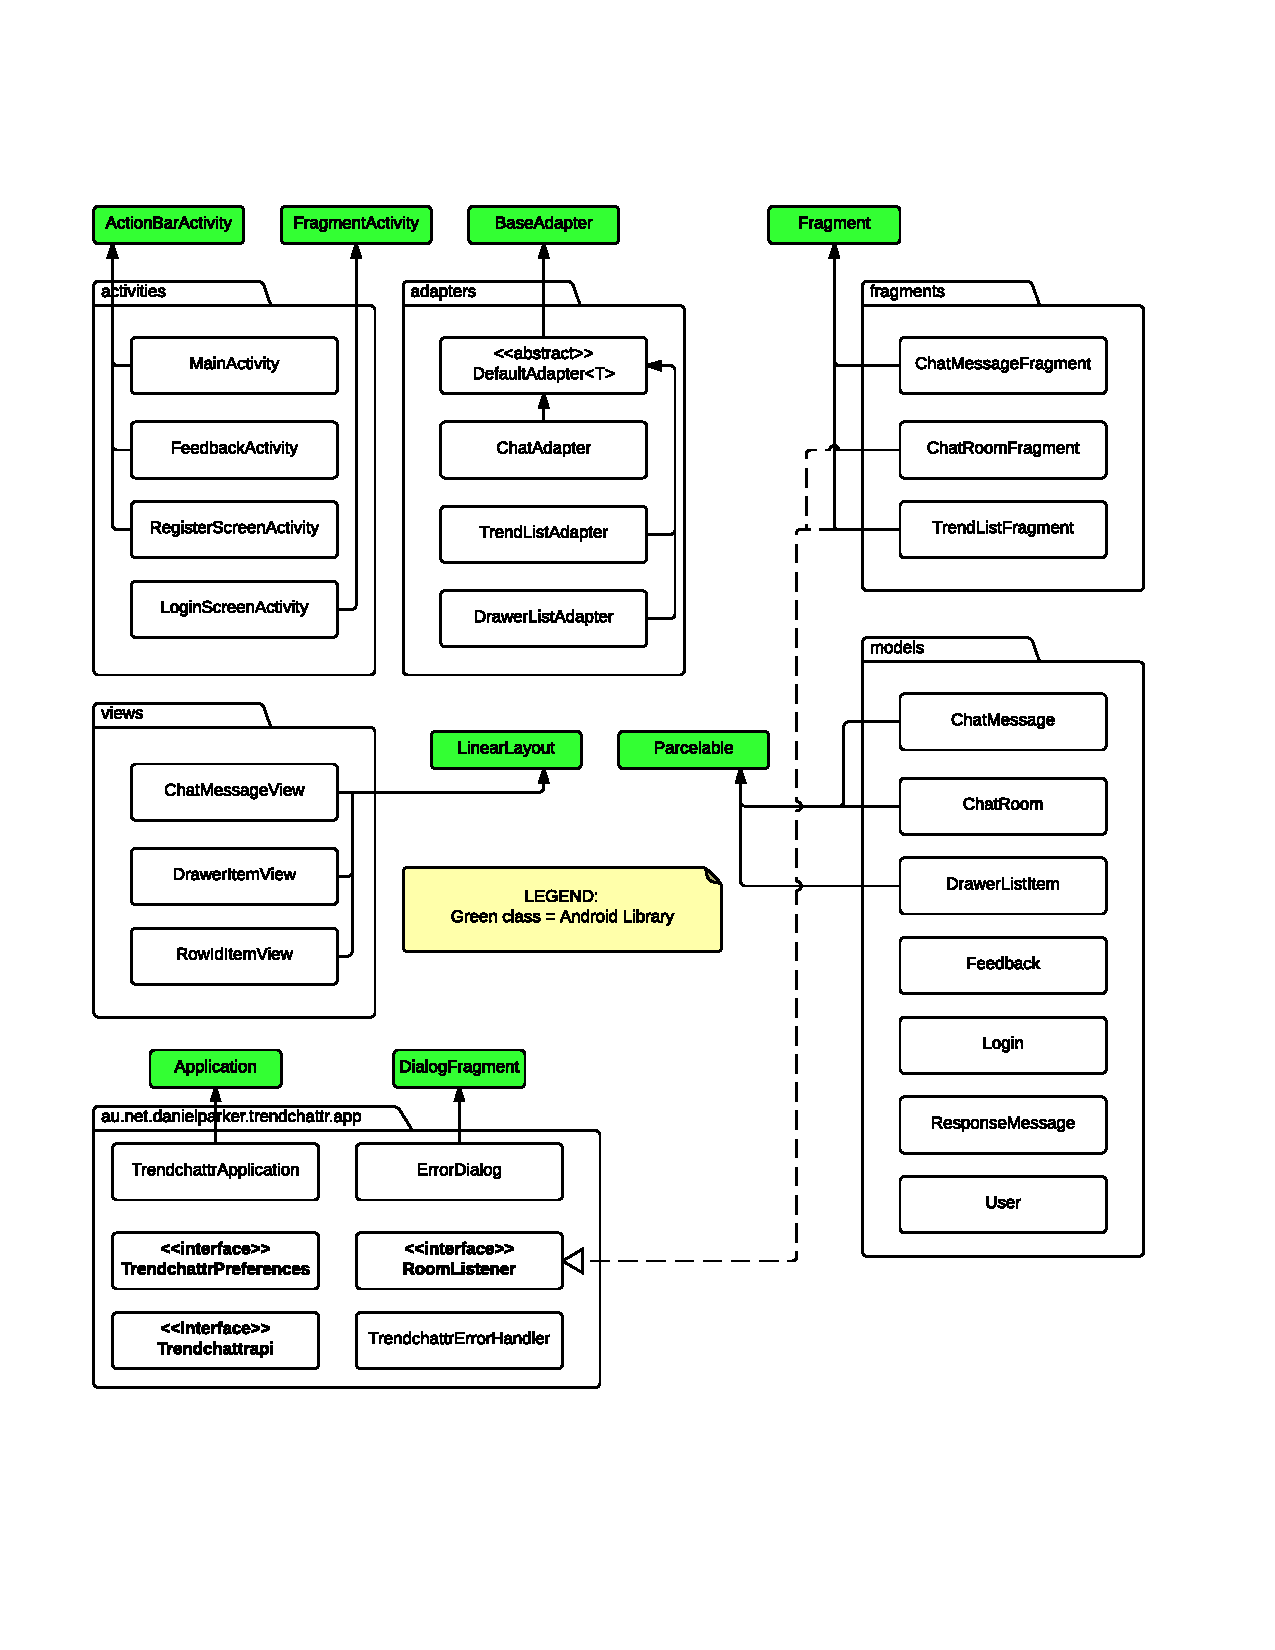
\includegraphics[width=\textwidth]{classes.pdf}}
      }
    \end{figure}
    %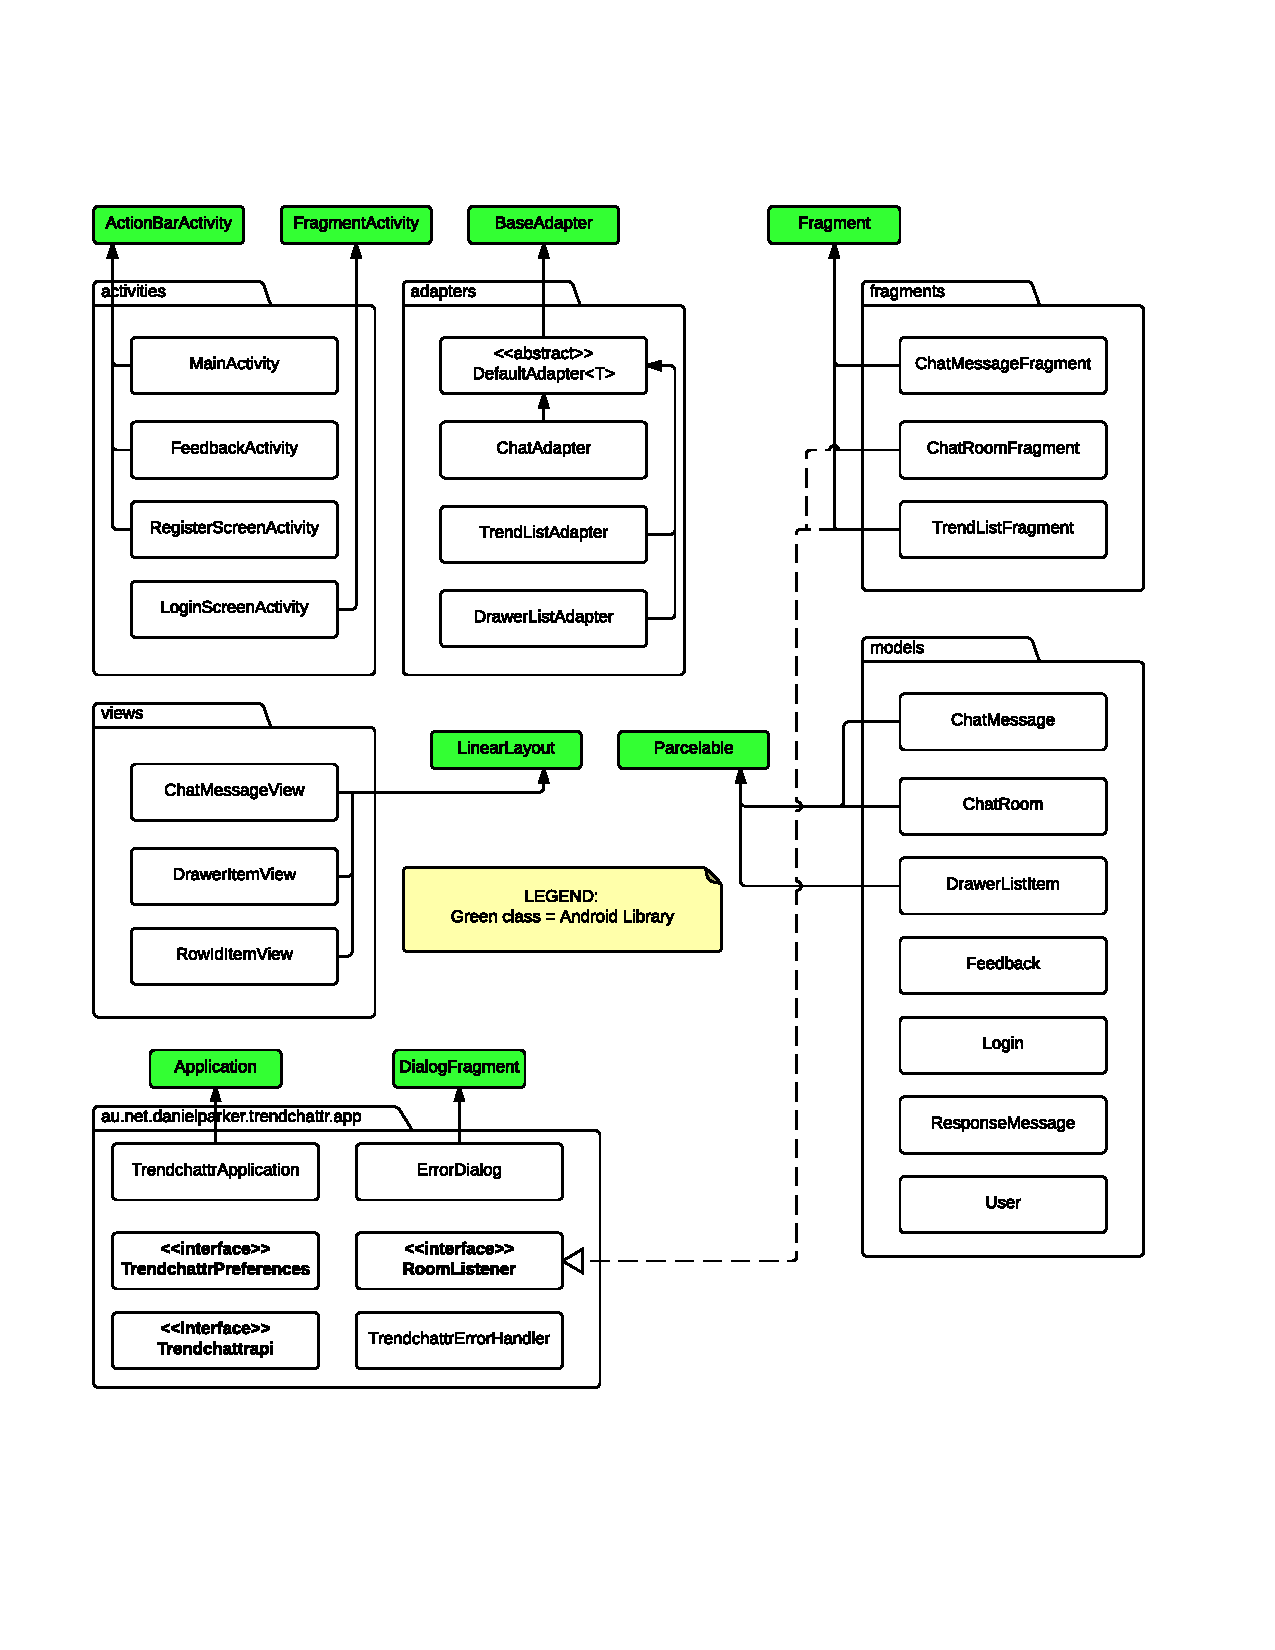
\includepdf[pages={1}]{classes.pdf}
  \subsection{Data Model}
  \begin{figure}[H]
    \centering{
      \fbox{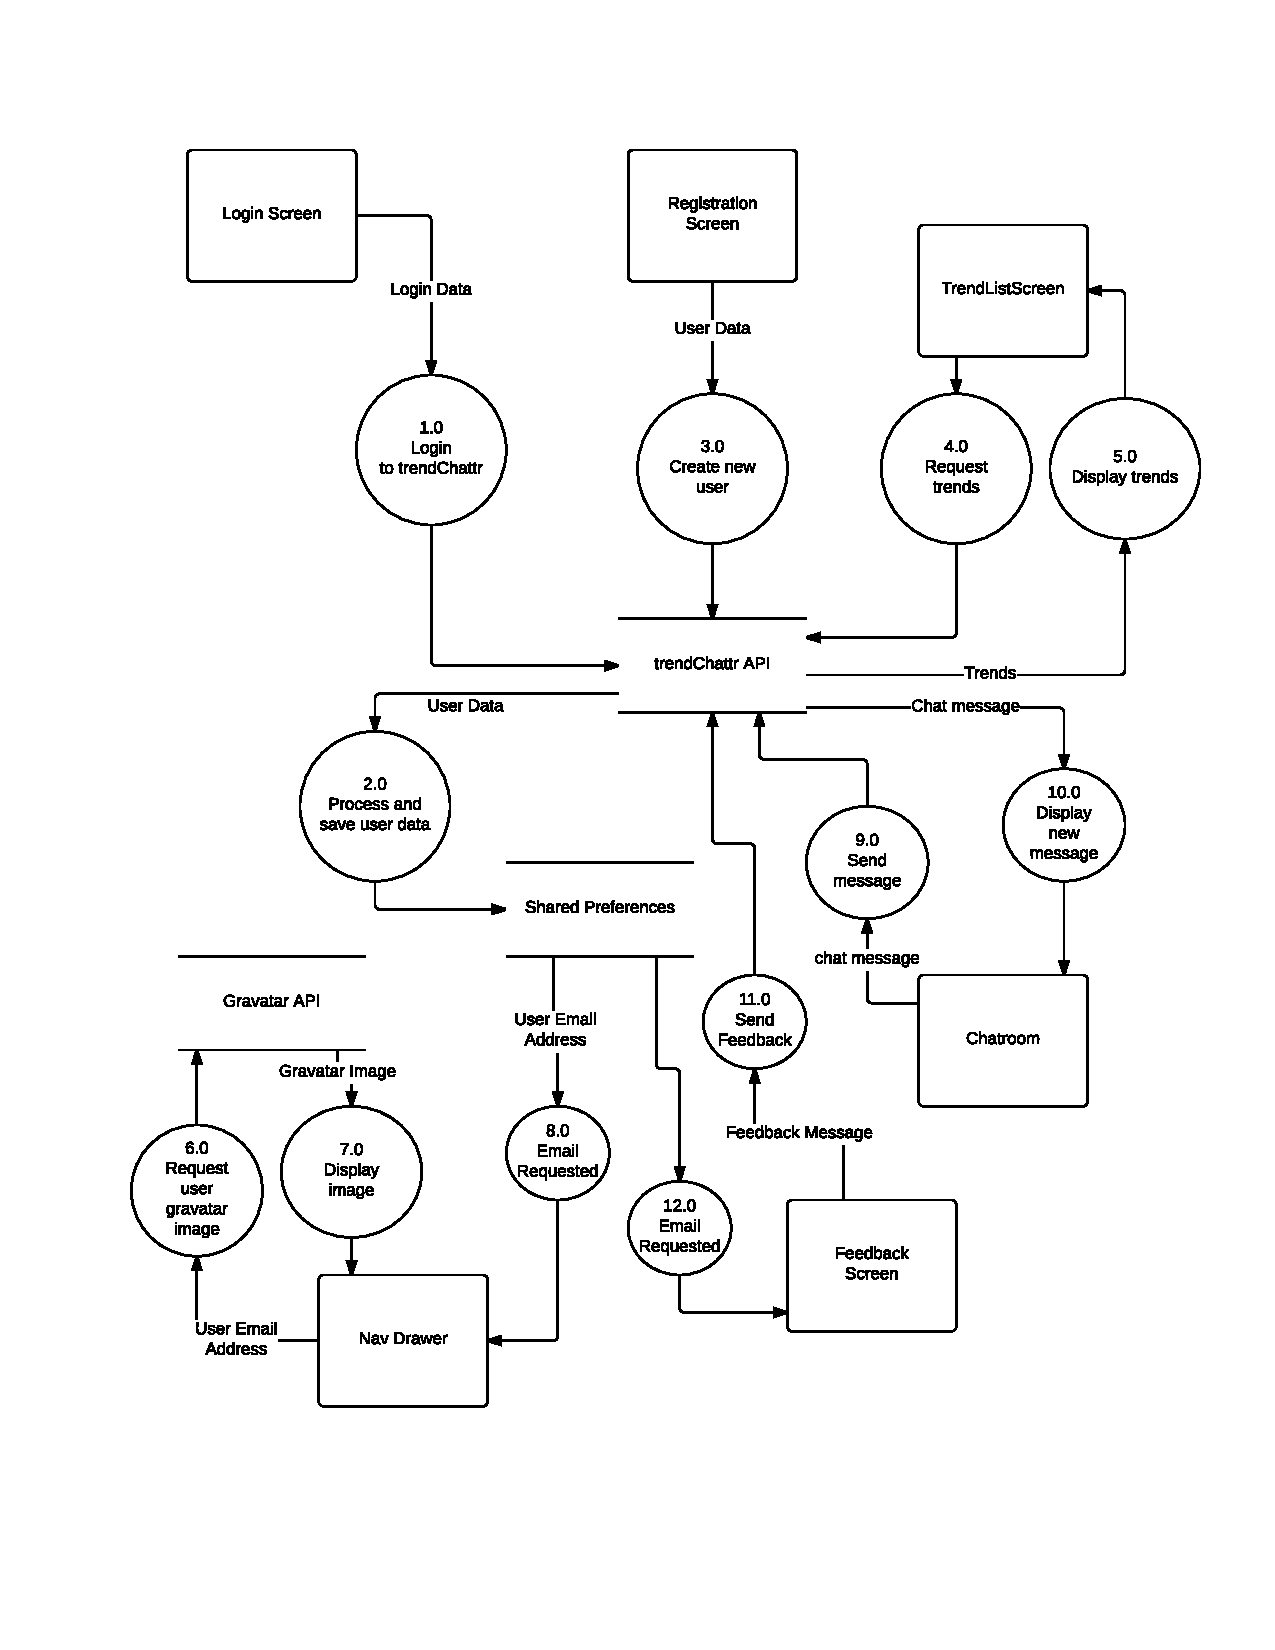
\includegraphics[width=\textwidth]{dataflow.pdf}}
    }
  \end{figure}
    %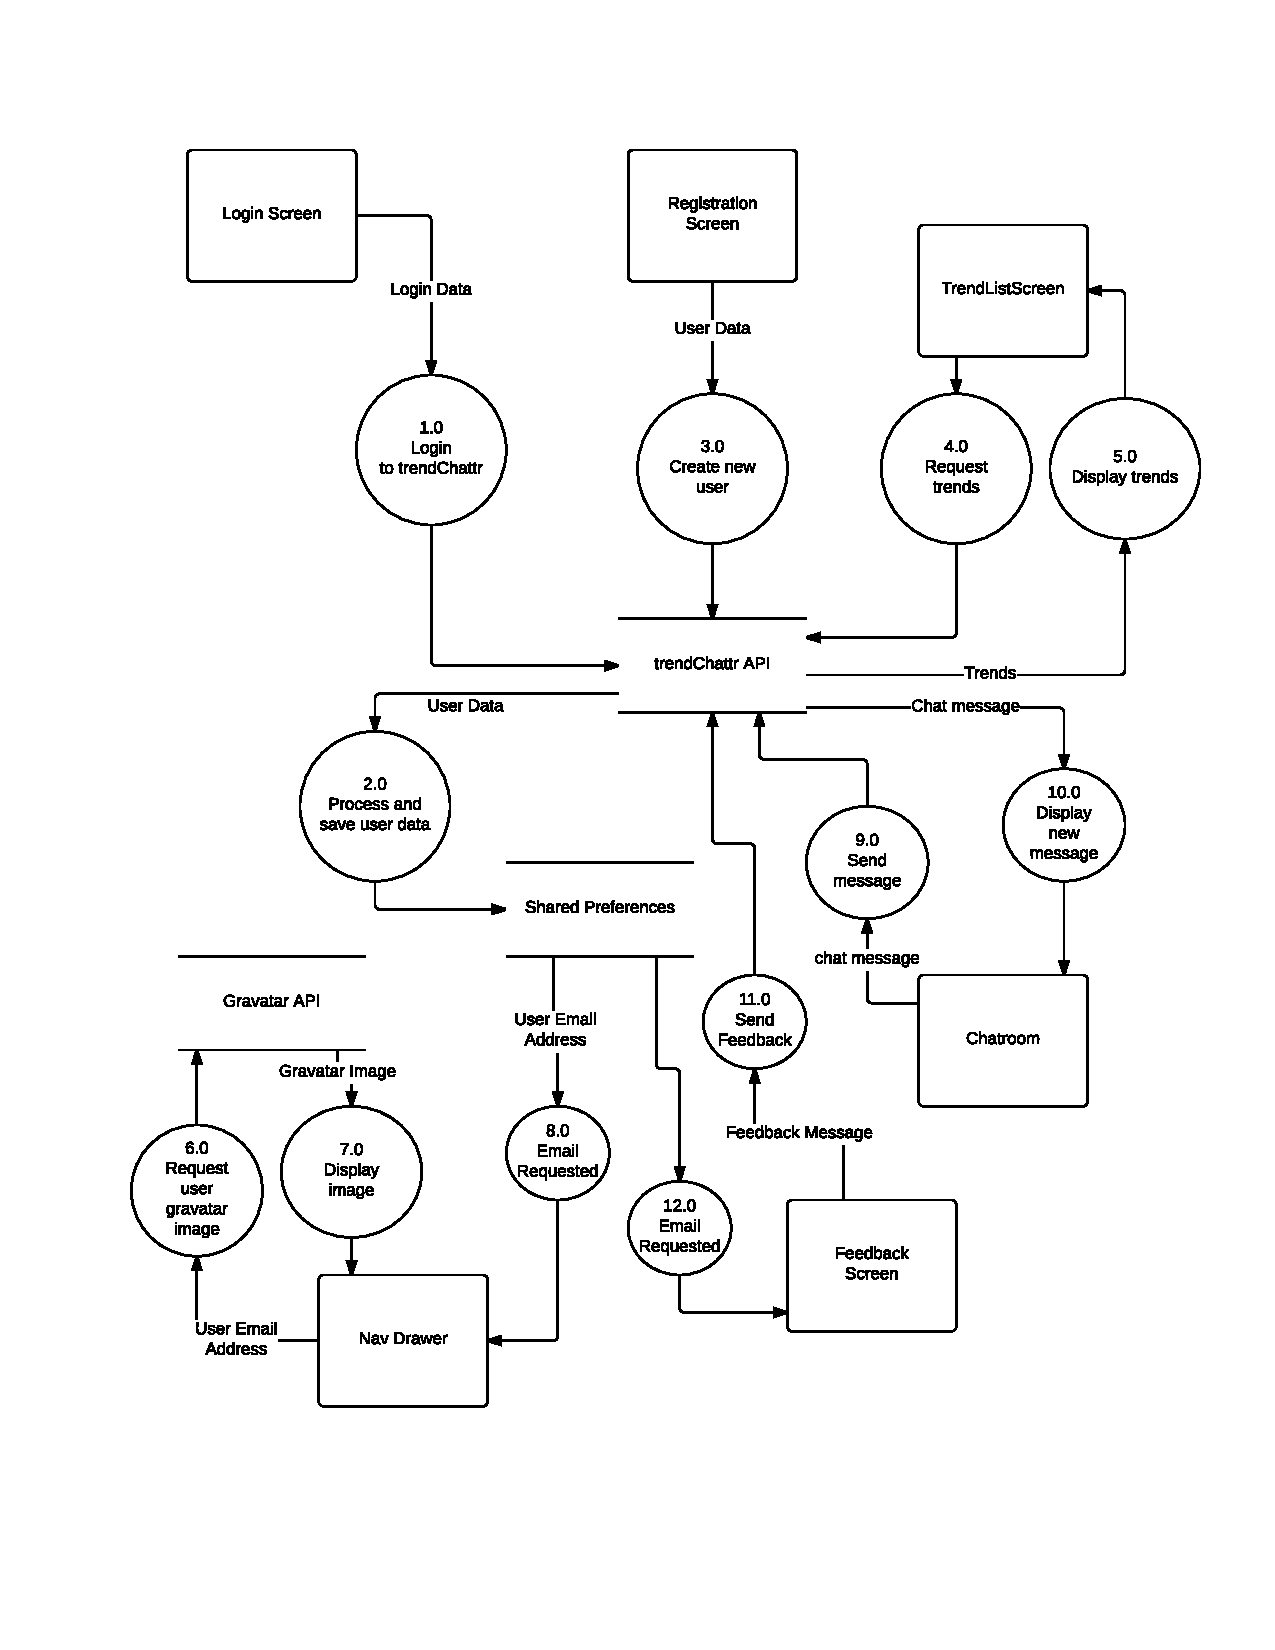
\includepdf[pages={1}]{dataflow.pdf}
\section{Visual Structure (Navigation)}
  \subsection{Navigation Flow Diagram}
    \begin{figure}[H]
      \centering{
        \fbox{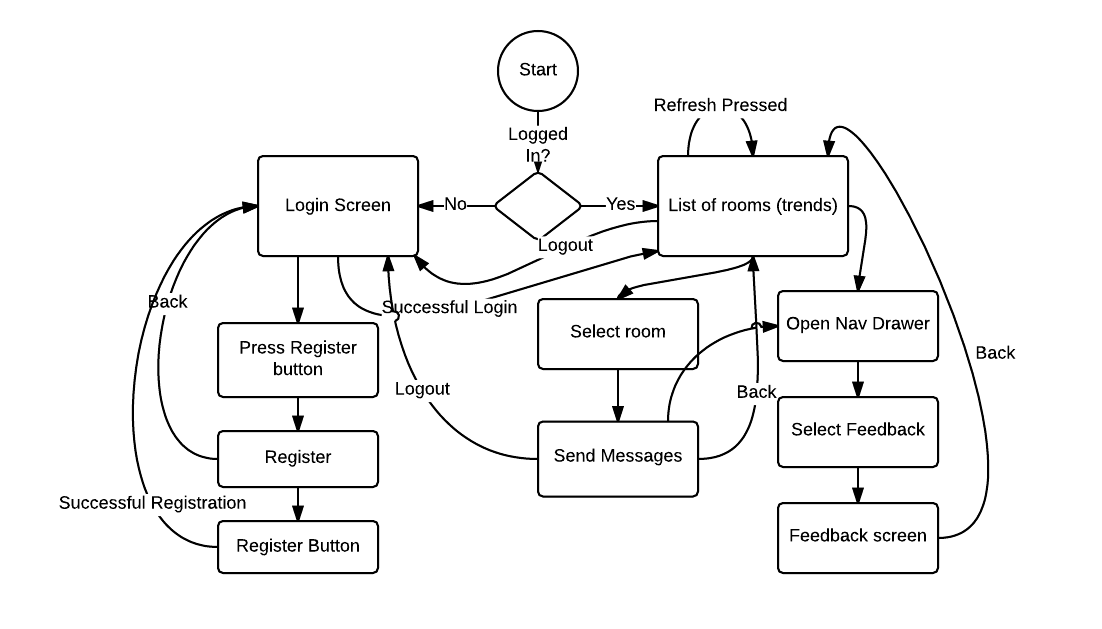
\includegraphics[width=\textwidth]{images/nav-flow.png}}
      }\\
    \end{figure}

\section{API Limitations}

\section{Summary}
  % Fill out
\section{References}
  % Fill out
\end{document}
